\section{The Peruvian power system}
\label{sec:peru}

\subsection{Market structure and generation mix}
\label{sec:peru:overview}

Following a macroeconomic collapse in the late 1980s, Peru moved from an integrated
state system to a competitive wholesale market with marginal nodal prices, capacity
payments and bilateral contracts. The Electric Concessions Law of 1992 unbundled
generation, transmission and distribution, and the supply auctions introduced from
2006 consolidated productivity gains, with clear efficiency improvements in
distribution after restructuring \citep{rudnick2019,perezreyes2009}.

The generation matrix remains dominated by hydropower and natural gas. By 2015 the
mix was roughly 50\,\% hydro and 45\,\% gas, with thermal sources overall accounting
for about 41\,\% of generation by 2017 \citep{rudnick2019}. The dependence is
structural: over half the natural gas consumed in the country goes to power plants
\citep{enerdata2024}, making electricity the primary driver of gas demand and
exposing it to price and supply shocks. Despite substantial solar, wind, geothermal
and biomass potential, non-conventional renewables supplied only about 5\,\% of
generation by 2022 \citep{campodonico2022}.

\citet{fiestas2024} find that raising non-conventional renewables to 28\,\% of the
matrix would cut gas consumption by \SI{2.04}{\kilo\meter\cubed} and avoid
\SI{4.99}{\mega\tonne} CO$_2$-eq annually while reducing system costs, and
\citet{delacruz2024} reach compatible conclusions to 2050. The economic case is
established; the route is not. The auction mechanism that for a decade channelled
renewable investment has been suspended, leaving developers without a reliable off-take
signal \citep{campodonico2022,torres2026}, and the grid was not built with variable
renewables in mind. This combination is not unusual: institutional quality and the cost
of capital, rather than resource quality, condition deployment
\citep{boateng2026,delrio2026}.

\subsection{Zonal structure and transmission}
\label{sec:peru:zones}

The model represents the system as three zones connected in series
(Figure~\ref{fig:map}). This is not a simplification for tractability but the
physical topology: Peru's main grid runs longitudinally, so the southern zone
reaches the rest of the system only through the centre. Table~\ref{tab:zones}
reports the January 2025 starting condition. The centre zone holds 60\,\% of
installed capacity; the Z1--Z2 and Z2--Z3 corridors provide \SI{900}{\mega\watt} and
\SI{700}{\mega\watt} of transfer capability; there is no direct Z1--Z3 path. A
series topology has no redundancy: a constraint on the central corridor isolates a
third of the system, and every transfer between the extremes consumes capacity on
both corridors.

\begin{figure}[tb]
  \centering
  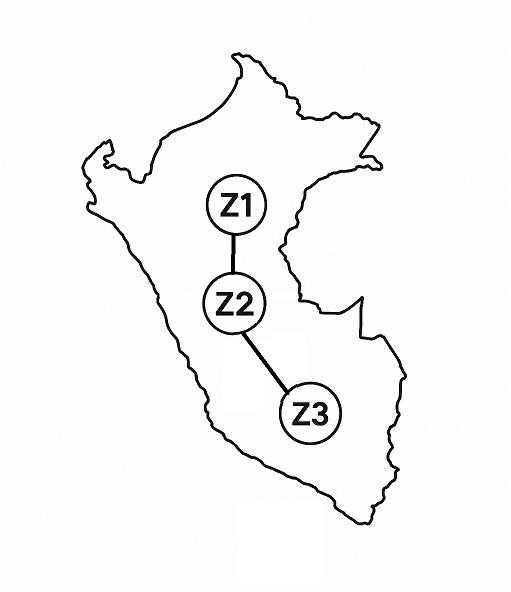
\includegraphics[width=0.40\textwidth]{mapa.png}
  \caption{Zonal representation of the Peruvian power system: north (Z1), centre
  (Z2) and south (Z3) in series. All exchange between the extremes transits the
  centre.}
  \label{fig:map}
\end{figure}

\begin{table}[tb]
  \centering
  \caption{Initial condition, January 2025, as represented in the model. Technology
  shares are given in Supplementary Material~S2.}
  \label{tab:zones}
  \small
  \begin{tabular}{@{}llrr@{}}
    \toprule
    Zone & Description & Capacity [\si{\mega\watt}] & Share \\
    \midrule
    Z1 & North   & \num{1606.1} & 11.4\,\% \\
    Z2 & Centre  & \num{8461.9} & 60.2\,\% \\
    Z3 & South   & \num{3989.0} & 28.4\,\% \\
    \midrule
    \multicolumn{2}{@{}l}{\textbf{Total}} & \textbf{\num{14057.0}} & 100\,\% \\
    \midrule
    \multicolumn{4}{@{}l}{\emph{Corridors:} Z1--Z2 \SI{900}{\mega\watt} over
      \SI{232.3}{\kilo\meter}; Z2--Z3 \SI{700}{\mega\watt} over \SI{271.8}{\kilo\meter}} \\
    \multicolumn{4}{@{}l}{\emph{Network:} \SI{16180}{\kilo\meter} total;
      thermal and reservoir hydro are 78\,\% of capacity, wind and solar 10.7\,\%} \\
    \bottomrule
  \end{tabular}
\end{table}

Congestion management in Peruvian planning has become more sophisticated, with
$n-1$ contingency screening alongside demand, generation, fuel-price and weather
projections \citep{valdivia2024}. At regional level, Andean interconnection is
technically and economically feasible but has stalled on regulatory sovereignty
rather than engineering \citep{sempertegui2017,guliev2022}.

\subsection{Planning challenges and the modelling implication}
\label{sec:peru:delays}

The gains from the 1990s reform were real but uneven. Once the initial wave of
privatisation ran its course, investment in generation and transmission slowed
considerably, indicating that the regulatory framework was not generating the
long-term certainty infrastructure capital requires \citep{rudnick2019}. The
suspension of the auction mechanism has hit onshore wind hardest: projects conceived
for structured procurement now compete in a spot market under price uncertainty,
and the best wind resources remain far from consumption \citep{torres2026}. Fossil
dependence and a renewable share of roughly 5.5\,\% of total energy leave Peru
exposed to external price swings \citep{colinacalvo2024}.

This is the feature that motivates the modelling choice in
Section~\ref{sec:methodology}. Lead times here are an institutional outcome rather
than an engineering parameter, and they differ systematically between generation,
which responds to a market signal, and transmission, which is planned centrally and
delivered on a longer clock. Representing that asymmetry explicitly is what allows
the model to be asked which of the two binds.

Peru is instructive comparatively: simultaneously a reference case for successful
market reform and a cautionary example of its limits --- competition and improved
security of supply, but increasing fossil dependence and a high reserve margin
\citep{rudnick2019}; early leadership in renewable auctions, but no consolidated
transition strategy, a gap visible against Chile, which started from a comparable base
and has moved further \citep{reyes2025,guliev2022}.
